\documentclass[../../main.tex]{subfiles}
\begin{document}

\paragraph{【新課程】}
{\bf [解]}
\subparagraph{(i)}
行列$A =
\begin{pmatrix} 0 & a \\ 1 & b
\end{pmatrix}$について，ケーリー・ハミルトンの定理より
\begin{align}
  A^2 - bA - aI = O \Longleftrightarrow A^2 = aI + bA
  \label{eq:1976-6new-ch}
\end{align}
が成り立つ．
$R$に属する任意の$2$つの行列を$X_1 = x_1 I + y_1 A$，$X_2 = x_2 I + y_2 A$（$x_1, y_1, x_2, y_2$は実数）とする．
単位行列$I$は任意の行列と可換（$IA = AI = A$，$I^2 = I$）であるから，その積$X_1 X_2$を展開すると
\begin{align}
  X_1 X_2 &= (x_1 I + y_1 A)(x_2 I + y_2 A) \nonumber\\
  &= x_1 x_2 I + (x_1 y_2 + y_1 x_2) A + y_1 y_2 A^2
\end{align}
となる．ここに\eqref{eq:1976-6new-ch}を代入すると
\begin{align}
  X_1 X_2 &= x_1 x_2 I + (x_1 y_2 + y_1 x_2) A + y_1 y_2 (aI + bA) \nonumber\\
  &= (x_1 x_2 + a y_1 y_2) I + (x_1 y_2 + y_1 x_2 + b y_1 y_2) A
\end{align}
となる．$x_1 x_2 + a y_1 y_2$および$x_1 y_2 + y_1 x_2 + b y_1 y_2$はいずれも実数であるから，$X_1 X_2$も$xI+yA$の形に表される．
したがって，$X_1 X_2 \in R$であり，題意は示された．

\subparagraph{(ii)}
$X = xI + yA \in R$を成分で表すと
\begin{align}
  X &= x
  \begin{pmatrix} 1 & 0 \\ 0 & 1
  \end{pmatrix} + y
  \begin{pmatrix} 0 & a \\ 1 & b
  \end{pmatrix} \nonumber\\
  &=
  \begin{pmatrix} x & ay \\ y & x + by
  \end{pmatrix}
\end{align}
である．$X = O \Longleftrightarrow x = y = 0$であるから，
\begin{align}
  G = \{ xI + yA \mid (x, y) \neq (0, 0) \}
\end{align}
である．行列$X$が逆行列をもつための必要十分条件は，行列式が$0$でないこと，すなわち$\det X \neq 0$である．
$X$の行列式を計算すると
\begin{align}
  \det X = x(x + by) - ay \cdot y = x^2 + bxy - ay^2
\end{align}
である．
したがって，$G$に属する任意の行列が逆行列をもつ条件は，$(x, y) \neq (0, 0)$を満たすすべての実数対$(x, y)$に対して
\begin{align}
  x^2 + bxy - ay^2 \neq 0
\end{align}
が成り立つこと，すなわち$x^2 + bxy - ay^2 = 0$を満たす実数解が$(x, y) = (0, 0)$に限られることである．
\begin{itemize}
  \item $y = 0$のとき: $x^2 = 0 \Longleftrightarrow x = 0$となり，解は$(0, 0)$のみである．
  \item $y \neq 0$のとき: 両辺を$y^2$で割り，$t = \dfrac{x}{y}$とおくと，$t$の$2$次方程式
    \begin{align}
      t^2 + bt - a = 0
    \end{align}
    が得られる．これが実数解をもたないことが必要十分である．
\end{itemize}
したがって，判別式を$D$とすると
\begin{align}
  D = b^2 - 4 \cdot 1 \cdot (-a) = b^2 + 4a < 0 \Longleftrightarrow a < -\dfrac{1}{4}b^2
\end{align}
である．
ゆえに，求める点$(a, b)$の範囲は
\begin{align}
  a < -\dfrac{1}{4}b^2 \tag{答}
\end{align}
であり，これを図示すると下図の斜線部分となる（境界線は含まない）．

\begin{figure}[h]
  \centering
  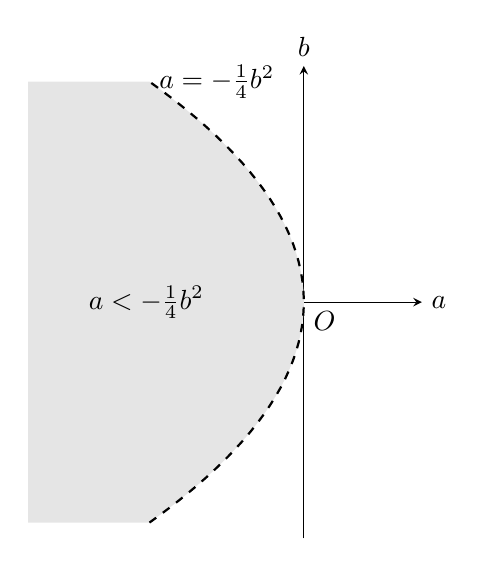
\begin{tikzpicture}[scale=1.0, >=stealth]
    \draw[->] (-3.5,0) -- (1.5,0) node[right] {$a$};
    \draw[->] (0,-3.0) -- (0,3.0) node[above] {$b$};
    \node[below right] at (0,0) {$O$};

    \fill[gray!20, domain=-2.8:2.8, samples=50] plot ({-0.25*\x*\x}, \x) -- (-3.5, 2.8) -- (-3.5, -2.8) -- cycle;
    \draw[thick, dashed, domain=-2.8:2.8, samples=50] plot ({-0.25*\x*\x}, \x);
    \node[right] at (-1.96, 2.8) {$a = -\frac{1}{4}b^2$};
    \node at (-2.0, 0) {$a < -\frac{1}{4}b^2$};
  \end{tikzpicture}
  \caption{点$(a, b)$の存在範囲（斜線部，境界線は含まない）}
\end{figure}

\paragraph{【旧課程】}
{\bf [解]}
\subparagraph{(i)}
方程式$f(x) = 0$の相異なる$4$実根を$\alpha_1 < \alpha_2 < \alpha_3 < \alpha_4$とする．
最高次の係数が$1$であるから
\begin{align}
  f(x) = (x - \alpha_1)(x - \alpha_2)(x - \alpha_3)(x - \alpha_4)
\end{align}
と因数分解される．
実数$k$に対して方程式$F(x) = f(x) + kf'(x) = 0$の実根の個数を調べる．

$1^\circ$ $k = 0$のとき:
$F(x) = f(x) = 0$であるから，実根は$\alpha_1, \alpha_2, \alpha_3, \alpha_4$の$4$個である．

$2^\circ$ $k \neq 0$のとき:
$x = \alpha_i$ ($i = 1, 2, 3, 4$)のとき，$f(\alpha_i) = 0$かつ$f'(\alpha_i) \neq 0$（重根をもたないため）であるから，$F(\alpha_i) = kf'(\alpha_i) \neq 0$となり，$\alpha_i$は$F(x) = 0$の根ではない．
したがって，$x \neq \alpha_i$のもとで両辺を$kf(x)$で割ると，
\begin{align}
  f(x) + kf'(x) = 0 \Longleftrightarrow \dfrac{f'(x)}{f(x)} = -\dfrac{1}{k}
\end{align}
と同値である．ここで
\begin{align}
  h(x) = \dfrac{f'(x)}{f(x)} = \sum_{i=1}^4 \dfrac{1}{x - \alpha_i}
\end{align}
とおく．各開区間$(-\infty, \alpha_1)$，$(\alpha_1, \alpha_2)$，$(\alpha_2, \alpha_3)$，$(\alpha_3, \alpha_4)$，$(\alpha_4, \infty)$において，
\begin{align}
  h'(x) = -\sum_{i=1}^4 \dfrac{1}{(x - \alpha_i)^2} < 0
\end{align}
であるから，$h(x)$はこれらの各区間で単調に減少する．
\begin{itemize}
  \item 各区間$(\alpha_i, \alpha_{i+1})$ ($i = 1, 2, 3$)において:
    $\lim_{x \to \alpha_i + 0} h(x) = +\infty$かつ$\lim_{x \to \alpha_{i+1} - 0} h(x) = -\infty$であるから，中間値の定理および単調性より，実数$-\dfrac{1}{k}$に対して$h(x) = -\dfrac{1}{k}$は各区間にただ$1$つの実根をもつ（計$3$個）．
  \item 区間$(-\infty, \alpha_1)$において:
    $\lim_{x \to -\infty} h(x) = 0$，$\lim_{x \to \alpha_1 - 0} h(x) = -\infty$であるから，$h(x)$は負の実数全体を値域とする．
    したがって，$k > 0$（$-\dfrac{1}{k} < 0$）のとき，この区間にただ$1$つの実根をもつ．
  \item 区間$(\alpha_4, \infty)$において:
    $\lim_{x \to \alpha_4 + 0} h(x) = +\infty$，$\lim_{x \to \infty} h(x) = 0$であるから，$h(x)$は正の実数全体を値域とする．
    したがって，$k < 0$（$-\dfrac{1}{k} > 0$）のとき，この区間にただ$1$つの実根をもつ．
\end{itemize}
$F(x)$は$4$次多項式であるから，実根は高々$4$個である．
以上より，$k > 0$のときも$k < 0$のときも実根はちょうど$4$個存在する．\casesend

よって，すべての実数$k$に対して実根の個数は
\begin{align}
  4\text{ 個} \tag{答}
\end{align}
である．

\subparagraph{(ii)}
$f(x) = x^4 + ax^3 + bx^2 + cx + d$について，
\begin{align}
  f'(x) &= 4x^3 + 3ax^2 + 2bx + c \nonumber\\
  f''(x) &= 12x^2 + 6ax + 2b = 12\left(x^2 + \dfrac{a}{2}x + \dfrac{b}{6}\right)
\end{align}
である．$f(x) = 0$と$f''(x) = 0$が共有する$2$つの相異なる実根を$r_1, r_2$ ($r_1 \neq r_2$)とする．
解と係数の関係より
\begin{align}
  r_1 + r_2 = -\dfrac{a}{2}
\end{align}
である．ここで，$x$軸方向に平行移動して$3$次の項を消去するため，
\begin{align}
  X = x + \dfrac{a}{4} \Longleftrightarrow x = X - \dfrac{a}{4}
\end{align}
とおく．このとき
\begin{align}
  \left(r_1 + \dfrac{a}{4}\right) + \left(r_2 + \dfrac{a}{4}\right) = r_1 + r_2 + \dfrac{a}{2} = 0
\end{align}
であるから，$R_1 = r_1 + \dfrac{a}{4}$とおけば，$R_2 = r_2 + \dfrac{a}{4} = -R_1$である．
$r_1 \neq r_2$より$R_1 \neq 0$であるから，$p = R_1 \neq 0$とおくと，共有根は$X = \pm p$と表される．
$X$の関数として$F(X) = f\left(X - \dfrac{a}{4}\right)$とおくと，$F(X)$の$3$次の係数は$0$であるから，実数$B, C, D$を用いて
\begin{align}
  F(X) = X^4 + BX^2 + CX + D
\end{align}
とおける．このとき
\begin{align}
  F''(X) = 12X^2 + 2B
\end{align}
である．$F''(X) = 0$の根が$X = \pm p$であるから，
\begin{align}
  12p^2 + 2B = 0 \Longleftrightarrow B = -6p^2
\end{align}
である．
また，$X = \pm p$は$F(X) = 0$の根でもあるから，$F(p) = 0$かつ$F(-p) = 0$が成り立つ．
これらを代入すると
\begin{align}
  \begin{cases}
    F(p) = p^4 + Bp^2 + Cp + D = -5p^4 + Cp + D = 0 \\
    F(-p) = p^4 + Bp^2 - Cp + D = -5p^4 - Cp + D = 0
  \end{cases}
\end{align}
である．辺々を引くと
\begin{align}
  2Cp = 0
\end{align}
を得る．$p \neq 0$であるから，$C = 0$である．
したがって
\begin{align}
  F(X) = X^4 + BX^2 + D
\end{align}
となり，$F(X)$は偶関数であるから，すべての$X$に対して
\begin{align}
  F(-X) = F(X)
\end{align}
が成り立つ．もとの変数$x$に戻せば，
\begin{align}
  f\left(-\dfrac{a}{4} - X\right) = f\left(-\dfrac{a}{4} + X\right)
\end{align}
が任意の$X$について成り立つことを意味する．
したがって，曲線$y = f(x)$は直線
\begin{align}
  x = -\dfrac{a}{4}
\end{align}
に関して線対称である．この直線は$y$軸に平行であるから，題意は示された．

\end{document}
